\documentclass[10pt,letterpaper,subeqn, xcolor=table]{beamer}

\setbeamertemplate{navigation symbols}{}
\usefonttheme{serif}
\usecolortheme{seahorse}


\usepackage[english]{babel}
\selectlanguage{english}
\usepackage{bm}
\usepackage{booktabs}
\usepackage{xcolor,colortbl}
\definecolor{dblue}{rgb}{0.,0.,0.6}
\usepackage{color}
\usepackage[update,prepend]{epstopdf}
\usepackage{framed}
\usepackage{fleqn}
\usepackage{graphics}
\usepackage{hyperref}
\usepackage[utf8]{inputenc}
\usepackage{setspace}
\usepackage{textcomp}
\usepackage{wrapfig}
\usepackage{multirow}
\usepackage{caption}
\usepackage{subcaption}
\usepackage{subfloat}
\setbeamertemplate{caption}[numbered]
\usepackage{wrapfig}



\usepackage{soul}
\definecolor{green1}{rgb}{0.5, 1, 0.3}

\usepackage{pgf,tikz}
\usepackage{pgfplots}
\usetikzlibrary{decorations}


\begin{document}
\title{Maternal Education and Maternal Mortality}
\subtitle{Evidence from a Large Panel and Various Natural Experiments}
\author{Sonia Bhalotra\inst{1} \and Damian Clarke\inst{2}}
\institute{\inst{1} University of Essex \and \inst{2} University of Santiago de Chile}
\date{\today}


\begin{frame}
\titlepage
\end{frame}

\frame{\frametitle{Take Away Points}
\begin{enumerate}
\item The probability that a mother dies in child birth is negatively related to her education \\ \vspace{2mm}
\item This finding is robust: it turns up in `long' panel data and in micro data from plausibly exogenous increases in education \\ \vspace{2mm}
\item The relevant margin is \emph{extensive}: moving from 0 to 1 years of education reduces maternal mortality ratio (MMR) by 166 per 100,000 live births \\ \vspace{2mm}
\item But smaller effects from intensive changes: moving from 7 to 8 years reduces MMR by 20 per 100,000 live births
\end{enumerate}
}

\begin{frame}
\begin{figure}[!htbp]
  \begin{center}
    \caption{Changes in Education and Changes in Maternal Mortality}
    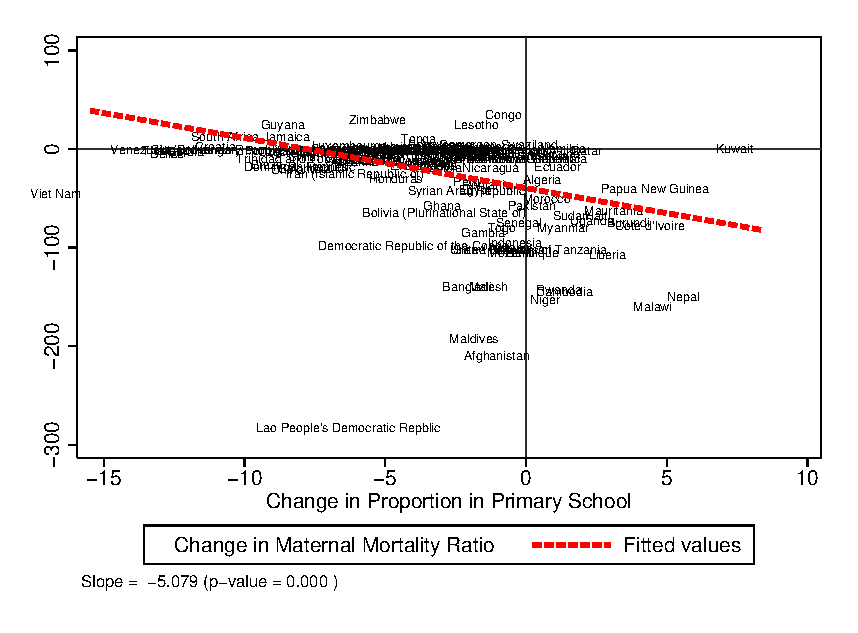
\includegraphics[scale=0.7]{./figures/MMReducPDeltas.eps}
  \end{center}
\end{figure}
\end{frame}



\section{Motivation}
\begin{frame}
\begin{center}
\Large	
\textsc{\textcolor{dblue}{Motivation}}
\end{center}
\end{frame}

\frame{\frametitle{Introduction}
\begin{itemize}
\item Every day 830 women die from preventable causes related to pregnancy and childbirth (WHO 2012)
\item MMR in developing countries is 240 per 100,000 live births, compared with 16 per 100,000 in developed
\item `Main sources' of maternal mortality: 
\begin{itemize}
\item Poverty 
\item Limited access to public services
\item Cultural practices
\item Lack of information
\end{itemize}
\item This paper: Does education play a role in maternal mortality rates?
\end{itemize}
}

\frame{\frametitle{Health and Education}
There is a lively literature in economics that documents a positive correlation between 
education and other indicators of health
\vspace{6mm}
\begin{itemize}
\item Smoking and drinking less, likelihood of prenatal care, adoption of new drugs (Cutler, Currie, Lleras-Muney among others)\ldots
\item Consistent with education conferring efficacy in acquiring and processing information (Rosenzweig, 1995)
\item Education may also influence health via income, though results generally hold conditional on income
\end{itemize}
}

\frame{\frametitle{This Paper}
Despite these well-studied relationships, both academic and policy literature have
very little to say about the link between education and maternal mortality.
\vspace{6mm}
\begin{itemize}
\item We examine whether there is a causal relationship between education and MMR
\item We identify using
\begin{enumerate}
\item A large panel, and 
\item A number of country-specific policy experiments
\end{enumerate}
\item We find consistent evidence to suggest that education has played an \emph{important and sizeable}
role in recent reductions of the MMR
\end{itemize}
}

\section{Identification}
\begin{frame}
\begin{center}
\Large	
\textsc{\textcolor{dblue}{Identification}}
\end{center}
\end{frame}

\begin{frame}
\frametitle{Panel}
We run the following on a panel of 108 countries from 1990-2010:
\vspace{5mm}
\begin{equation}
\label{eqn:panel}
MMR_{it}=\alpha_i+\mathbf{educ}_{it}\beta + \mathbf{W}_{it}\gamma+\delta_t+\varepsilon_{it},
\end{equation}
\vspace{5mm}
\begin{itemize}
\item We are intersted in $\hat\beta$, which is identified under typical (fixed-effect) panel assumptions
\item Include a continously more demanding set of time-varying controls $\mathbf{W}_{it}$, linear trends
\item Examine various functional forms and measures of female education (conditional and unconditional on male education)
\end{itemize}
\end{frame}

\begin{frame}[label=ID]
\frametitle{Country-Specific Reforms}
However, we may be concerned that additional time-varying factors are omitted from (\ref{eqn:panel}). So:
\begin{eqnarray}
 \label{eqn:Nigeria}
 y_{ijk}&=&\alpha + \beta \text{ UPE Cohort}_{jk}+\gamma \text{UPE Input}_k+ \\ \nonumber
& & \delta(\text{UPE Input}_k\times\text{UPE Cohort}_{jk})+\textbf{X}^\prime_{ijk}\theta+\varepsilon_{ijk}. \\
\nonumber
\end{eqnarray}
\vspace{5mm}
We run similar regressions for a number of country-specific contexts:
\begin{itemize}
\item Nigeria (above): Universal Primary Education, 1976
\item \hyperlink{ZIMBABWE}{\textcolor{blue}{Zimbabwe}}: Extensions of availability after independence, 1980
\item \hyperlink{KENYA}{\textcolor{blue}{Kenya}}: Rearrangement of years to obtain KCPE, 1985
\end{itemize}
\end{frame}


\section{Data}
\begin{frame}
\begin{center}
\Large	
\textsc{\textcolor{dblue}{Data}}
\end{center}
\end{frame}

\begin{frame}[label=DATA]
\frametitle{Data}
We compile a cross-country dataset consisting of:
\begin{itemize}
\item educational outcomes from Barro and Lee (2010, 2013)
\item maternal mortality ratios (\hyperlink{MMRnote}{\textcolor{blue}{MMR}}) from WHO 2012
\item additional controls from World Bank Data Bank, and constructed from DHS (\hyperlink{SumStats}{\textcolor{blue}{Summary Statistics}})
\end{itemize}
\vspace{5mm}
For country-specific estimates we use the DHS:
\begin{itemize}
\item Education comes from female respondents of 4 or 5 waves of surveys in each country (\hyperlink{SumStatsCountry}{\textcolor{blue}{Summary Statistics}})
\item Maternal mortality is calculated by the sisterhood method
\item This allows us to calculate country sub-region averages by cohort
\end{itemize}
\end{frame}

\section{Results}
\begin{frame}
\begin{center}
\Large	
\textsc{\textcolor{dblue}{Results}}
\end{center}
\end{frame}


\begin{frame}
\begin{landscape}\begin{table}[htpb!]\begin{center}\caption{Cross-Country Results of MMR and Female Educational Attainment}\label{MMRtab:MMRpercent}\begin{tabular}{lcccccccc}\toprule&\begin{footnotesize}(1)\end{footnotesize}&\begin{footnotesize}(2)\end{footnotesize}&\begin{footnotesize}(3)\end{footnotesize}&\begin{footnotesize}(4)\end{footnotesize}&\begin{footnotesize}(5)\end{footnotesize}&\begin{footnotesize}(6)\end{footnotesize}&\begin{footnotesize}(7)\end{footnotesize}&\begin{footnotesize}(8) \end{footnotesize}\\
VARIABLES&MMR&MMR&MMR&MMR&MMR&MMR&MMR&MMR\\ \midrule
&&&&&&&&\\
Primary Education (\% Population) &-10.06***&-10.24***&-8.463***&-8.445***&-7.738***&-7.386***&-7.185***&-6.597***\\
&\begin{footnotesize}(1.407)\end{footnotesize}&\begin{footnotesize}(1.625)\end{footnotesize}&\begin{footnotesize}(1.556)\end{footnotesize}&\begin{footnotesize}(1.559)\end{footnotesize}&\begin{footnotesize}(1.641)\end{footnotesize}&\begin{footnotesize}(1.710)\end{footnotesize}&\begin{footnotesize}(2.068)\end{footnotesize}&\begin{footnotesize}(1.941)\end{footnotesize}\\
Secondary Education (\% Population) &-9.696***&-9.789***&-6.672***&-6.689***&-5.979***&-5.375***&-5.146***&-4.514***\\
&\begin{footnotesize}(1.214)\end{footnotesize}&\begin{footnotesize}(1.305)\end{footnotesize}&\begin{footnotesize}(1.376)\end{footnotesize}&\begin{footnotesize}(1.367)\end{footnotesize}&\begin{footnotesize}(1.432)\end{footnotesize}&\begin{footnotesize}(1.578)\end{footnotesize}&\begin{footnotesize}(1.872)\end{footnotesize}&\begin{footnotesize}(1.716)\end{footnotesize}\\
Tertiary Education (\% Population) &-9.521***&-10.35***&-4.618**&-4.741**&-4.501**&-4.126**&-4.061**&-3.651**\\
&\begin{footnotesize}(1.238)\end{footnotesize}&\begin{footnotesize}(1.412)\end{footnotesize}&\begin{footnotesize}(2.035)\end{footnotesize}&\begin{footnotesize}(1.968)\end{footnotesize}&\begin{footnotesize}(1.854)\end{footnotesize}&\begin{footnotesize}(1.928)\end{footnotesize}&\begin{footnotesize}(1.965)\end{footnotesize}&\begin{footnotesize}(1.833)\end{footnotesize}\\
year 1995&&&-11.36&-12.13&-4.635&-4.217&-2.281&-7.504\\
&&&\begin{footnotesize}(12.82)\end{footnotesize}&\begin{footnotesize}(13.39)\end{footnotesize}&\begin{footnotesize}(12.28)\end{footnotesize}&\begin{footnotesize}(11.90)\end{footnotesize}&\begin{footnotesize}(14.28)\end{footnotesize}&\begin{footnotesize}(14.95)\end{footnotesize}\\
year 2000&&&-30.15*&-31.06*&-19.39&-16.87&-13.19&-16.39\\
&&&\begin{footnotesize}(17.38)\end{footnotesize}&\begin{footnotesize}(18.21)\end{footnotesize}&\begin{footnotesize}(16.56)\end{footnotesize}&\begin{footnotesize}(16.27)\end{footnotesize}&\begin{footnotesize}(21.04)\end{footnotesize}&\begin{footnotesize}(21.15)\end{footnotesize}\\
year 2005&&&-56.27**&-60.50**&-37.83&-37.68&-32.58&-28.84\\
&&&\begin{footnotesize}(22.49)\end{footnotesize}&\begin{footnotesize}(27.52)\end{footnotesize}&\begin{footnotesize}(24.31)\end{footnotesize}&\begin{footnotesize}(23.39)\end{footnotesize}&\begin{footnotesize}(29.22)\end{footnotesize}&\begin{footnotesize}(28.47)\end{footnotesize}\\
year 2010&&&-80.21***&-87.56**&-63.80*&-62.16*&-56.23&-42.41\\
&&&\begin{footnotesize}(27.81)\end{footnotesize}&\begin{footnotesize}(38.27)\end{footnotesize}&\begin{footnotesize}(33.73)\end{footnotesize}&\begin{footnotesize}(32.62)\end{footnotesize}&\begin{footnotesize}(38.68)\end{footnotesize}&\begin{footnotesize}(37.38)\end{footnotesize}\\
log GDP per capita&&&&8.223&5.817&9.654&8.563&5.675\\
&&&&\begin{footnotesize}(20.83)\end{footnotesize}&\begin{footnotesize}(20.45)\end{footnotesize}&\begin{footnotesize}(20.13)\end{footnotesize}&\begin{footnotesize}(19.69)\end{footnotesize}&\begin{footnotesize}(19.57)\end{footnotesize}\\
Immunization (DPT) &&&&&-2.194**&-2.022**&-1.978**&-1.950**\\
&&&&&\begin{footnotesize}(0.886)\end{footnotesize}&\begin{footnotesize}(0.880)\end{footnotesize}&\begin{footnotesize}(0.909)\end{footnotesize}&\begin{footnotesize}(0.913)\end{footnotesize}\\
Attended Births&&&&&&-1.275&-1.172&-1.451*\\
&&&&&&\begin{footnotesize}(0.813)\end{footnotesize}&\begin{footnotesize}(0.791)\end{footnotesize}&\begin{footnotesize}(0.804)\end{footnotesize}\\
Fertility&&&&&&&8.339&-5.573\\
&&&&&&&\begin{footnotesize}(25.38)\end{footnotesize}&\begin{footnotesize}(25.92)\end{footnotesize}\\
Teen births&&&&&&&&1.835**\\
&&&&&&&&\begin{footnotesize}(0.908)\end{footnotesize}\\
Constant&1,022***&1,044***&824.6***&764.7***&904.4***&915.6***&866.4***&795.2***\\
&\begin{footnotesize}(100.4)\end{footnotesize}&\begin{footnotesize}(113.8)\end{footnotesize}&\begin{footnotesize}(114.1)\end{footnotesize}&\begin{footnotesize}(205.4)\end{footnotesize}&\begin{footnotesize}(200.9)\end{footnotesize}&\begin{footnotesize}(191.9)\end{footnotesize}&\begin{footnotesize}(277.4)\end{footnotesize}&\begin{footnotesize}(289.2)\end{footnotesize}\\
&&&&&&&&\\
Observations&710&428&428&428&428&428&428&428\\
R-squared&0.344&0.450&0.489&0.490&0.519&0.529&0.529&0.542\\
Number of countries&142&108&108&108&108&108&108&108\\
\midrule
\multicolumn{9}{p{20cm}}{\begin{footnotesize}\textsc{Notes:} All regressions include fixed-effects by country. For the full list of countries by year see online appendix table 1.  Results are for the percent of the female population between the ages of  15 and 39 with each level of education in each country.  A full description of control variables is available in section \ref{scn:data}, and as the note to table \ref{MMRtab:sumstats}.  Standard errors clustered at the level of the country are diplayed.
$^{*}$p$<$0.1; $^{**}$p$<$0.05; $^{***}$p$<$0.01\end{footnotesize}} \\ \bottomrule 
\end{tabular}\end{center}\end{table}\end{landscape}

\end{frame}

\begin{frame}[label=GTABLE]
\begin{landscape}\begin{table}[htpb!]\begin{center}\caption{Cross-Country Results: MMR and Female versus Male Education}\label{MMRtab:MMRgender}\begin{tabular}{lcccccccc}\toprule&\begin{footnotesize}(1)\end{footnotesize}&\begin{footnotesize}(2)\end{footnotesize}&\begin{footnotesize}(3)\end{footnotesize}&\begin{footnotesize}(4)\end{footnotesize}&\begin{footnotesize}(5)\end{footnotesize}&\begin{footnotesize}(6)\end{footnotesize}&\begin{footnotesize}(7)\end{footnotesize}&\begin{footnotesize}(8) \end{footnotesize}\\
VARIABLES&MMR&MMR&MMR&MMR&MMR&MMR&MMR&MMR\\ \midrule
&&&&&&&&\\
Primary Education (\% Females) &-13.41***&-16.37***&-14.41***&-14.34***&-13.42***&-11.97***&-12.10***&-11.18**\\
&\begin{footnotesize}(2.576)\end{footnotesize}&\begin{footnotesize}(4.528)\end{footnotesize}&\begin{footnotesize}(4.311)\end{footnotesize}&\begin{footnotesize}(4.326)\end{footnotesize}&\begin{footnotesize}(4.310)\end{footnotesize}&\begin{footnotesize}(4.270)\end{footnotesize}&\begin{footnotesize}(4.348)\end{footnotesize}&\begin{footnotesize}(4.357)\end{footnotesize}\\
Secondary Education (\% Females) &-8.008***&-13.38***&-8.637**&-8.642**&-7.538**&-6.686*&-6.951*&-6.420*\\
&\begin{footnotesize}(2.402)\end{footnotesize}&\begin{footnotesize}(3.778)\end{footnotesize}&\begin{footnotesize}(3.980)\end{footnotesize}&\begin{footnotesize}(3.968)\end{footnotesize}&\begin{footnotesize}(3.692)\end{footnotesize}&\begin{footnotesize}(3.728)\end{footnotesize}&\begin{footnotesize}(3.740)\end{footnotesize}&\begin{footnotesize}(3.605)\end{footnotesize}\\
Tertiary Education (\% Females) &-7.481***&-10.69**&-0.0648&-0.145&-0.1000&0.289&0.231&0.171\\
&\begin{footnotesize}(2.648)\end{footnotesize}&\begin{footnotesize}(4.151)\end{footnotesize}&\begin{footnotesize}(6.655)\end{footnotesize}&\begin{footnotesize}(6.525)\end{footnotesize}&\begin{footnotesize}(5.774)\end{footnotesize}&\begin{footnotesize}(5.894)\end{footnotesize}&\begin{footnotesize}(5.867)\end{footnotesize}&\begin{footnotesize}(5.719)\end{footnotesize}\\
Primary Education (\% Males) &3.674&8.955&8.946&8.819&8.649*&7.618&7.668&7.195\\
&\begin{footnotesize}(3.487)\end{footnotesize}&\begin{footnotesize}(6.055)\end{footnotesize}&\begin{footnotesize}(5.511)\end{footnotesize}&\begin{footnotesize}(5.509)\end{footnotesize}&\begin{footnotesize}(5.199)\end{footnotesize}&\begin{footnotesize}(5.016)\end{footnotesize}&\begin{footnotesize}(5.027)\end{footnotesize}&\begin{footnotesize}(5.054)\end{footnotesize}\\
Secondary Education (\% Males) &-2.006&6.088&5.040&4.943&4.411&4.458&4.601&4.510\\
&\begin{footnotesize}(3.528)\end{footnotesize}&\begin{footnotesize}(5.270)\end{footnotesize}&\begin{footnotesize}(4.741)\end{footnotesize}&\begin{footnotesize}(4.766)\end{footnotesize}&\begin{footnotesize}(4.242)\end{footnotesize}&\begin{footnotesize}(4.230)\end{footnotesize}&\begin{footnotesize}(4.221)\end{footnotesize}&\begin{footnotesize}(4.198)\end{footnotesize}\\
Tertiary Education (\% Males) &-2.993&0.781&-3.526&-3.808&-3.570&-3.299&-3.287&-2.903\\
&\begin{footnotesize}(3.985)\end{footnotesize}&\begin{footnotesize}(5.931)\end{footnotesize}&\begin{footnotesize}(6.879)\end{footnotesize}&\begin{footnotesize}(6.897)\end{footnotesize}&\begin{footnotesize}(6.075)\end{footnotesize}&\begin{footnotesize}(6.152)\end{footnotesize}&\begin{footnotesize}(6.168)\end{footnotesize}&\begin{footnotesize}(6.086)\end{footnotesize}\\
&&&&&&&&\\Observations&710&428&428&428&428&428&428&428\\
R-squared&0.560&0.610&0.655&0.656&0.682&0.691&0.692&0.696\\
Number of countries&142&108&108&108&108&108&108&108\\
\midrule
\multicolumn{9}{p{20cm}}{\begin{footnotesize}\textsc{Notes:} All regressions include fixed-effects by country. For the full list of countries by year see table \ref{MMRtab:survey}. Educational variables are the same as those in table \ref{MMRtab:MMRpercent} however include both female and male figures for each variable (ages 15-39). A full description of control variables is available in section \ref{scn:data}, and as the note to table \ref{MMRtab:sumstats}.  Standard errors clustered at the level of the country are diplayed.
$^{*}$p$<$0.1; $^{**}$p$<$0.05; $^{***}$p$<$0.01\end{footnotesize}} \\ \bottomrule 
\end{tabular}\end{center}\end{table}\end{landscape}
\end{frame}

\begin{frame}
\frametitle{Education During Fertile Period Affects Maternal Mortality}
  \begin{figure}[!htbp]
\begin{center}
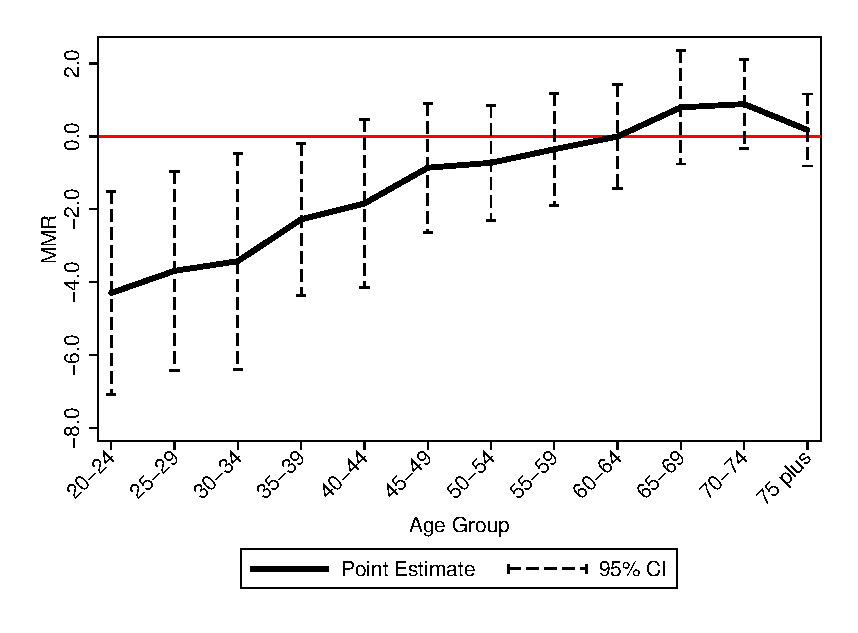
\includegraphics[scale=0.65]{./figures/PrimaryAge.eps}
\caption{Effect of Primary Education on MMR by Women's Age}
\end{center}
\end{figure}
\end{frame}


\begin{frame}[label=ZIMBABWE_EDUC]
\frametitle{Educational Reforms}
  \begin{figure}[!htbp]
\begin{center}
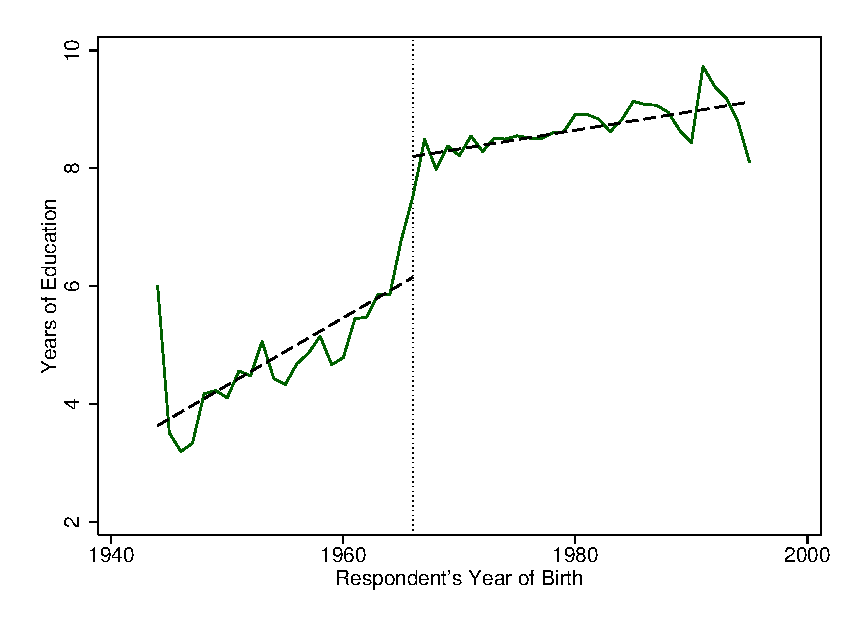
\includegraphics[scale=0.7]{./figures/Zimbabwe_educ.eps}
\caption{Educational Attainment by Cohort: Zimbabwe}
\end{center}
\end{figure}
\hyperlink{NIGERIA_EDUC}{\beamergotobutton{For Nigeria}}
\end{frame}

\begin{frame}[label=ZIMBABWE_MMR]
\frametitle{Educational Reforms}
  \begin{figure}[!htbp]
\begin{center}
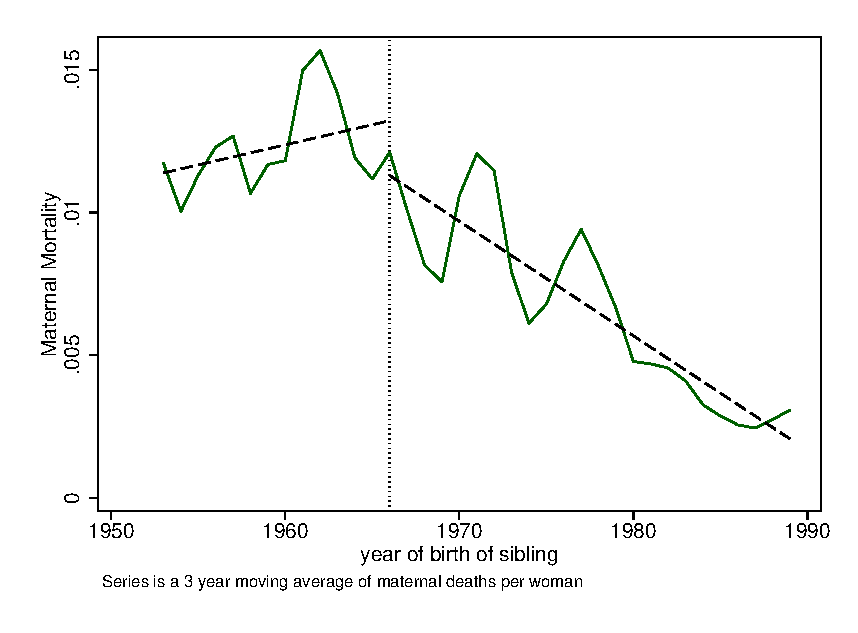
\includegraphics[scale=0.7]{./figures/Zimbabwe_mmr.eps}
\caption{Maternal Mortality by Cohort: Zimbabwe}
\end{center}
\end{figure}
\hyperlink{NIGERIA_MMR}{\beamergotobutton{For Nigeria}}
\end{frame}


\frame{\frametitle{Educational Reforms}
\begin{table}[htpb!]
\begin{center}
\scalebox{0.7}{
\begin{tabular}{lccc} \toprule
  & (1) & (2)  & (3) \\
  & Nigeria & Zimbabwe & Kenya \\
\midrule
\textsc{Panel A: Education} & & & \\
Treatment 1 & 2.179$^{***}$& 1.148$^{***}$& 0.953$^{***}$ \\
& \begin{footnotesize} (0.806)\end{footnotesize} & \begin{footnotesize} (0.167) \end{footnotesize}& \begin{footnotesize} (0.265) \end{footnotesize} \\
Treatment 2 & 1.059$^{**}$&& \\
&  \begin{footnotesize}(0.455) \end{footnotesize}&& \\
& & & \\
Observations & 12,735 &  10,195 & 13,703 \\ \midrule
\multicolumn{4}{l}{\textsc{Panel B: Maternal Mortality}}  \\
\rowcolor{green1} Treatment 1 & -0.0192$^{**}$& -0.00413$^{**}$& 0.00689 \\
& \begin{footnotesize} (0.00951) \end{footnotesize} & \begin{footnotesize} (0.00143)\end{footnotesize} & \begin{footnotesize} (0.00553) \end{footnotesize} \\
Treatment 2 & -0.0118$^{**}$&& \\
& \begin{footnotesize} (0.00518) \end{footnotesize} && \\
& & & \\
Observations & 28,694 &  28,631 & 25,602 \\ \bottomrule
        \multicolumn{4}{c}{\begin{footnotesize} *** p$<$0.01, ** p$<$0.05, * p$<$0.1\end{footnotesize}} \\
        \multicolumn{4}{p{9cm}}{\begin{footnotesize}\textsc{Notes:} Panel A is the first stage equation, panel B is reduced form. Full specifications and treatment variables are described in section 5.  Standard errors are clustered by state and birth cohort. `Treatment 2' refers to pre-treatment cohorts who are partially affected due to over-age enrolments. `Treatment 1' refers to affected cohorts. \end{footnotesize}} \\ \midrule

\end{tabular}
}
\end{center}
\end{table}
}

\frame{\frametitle{Country-Specific Results}
\begin{itemize}
\item Effects are significant in Nigeria, Zimbabwe
\begin{itemize}
 \item These are reforms which largely affect \emph{primary} or lower secondary enrolment 
 \item No effect found in Kenya (reform affects 7\textsuperscript{th} year of education)
\end{itemize}
\item By using data on fertility per woman (DHS), we can convert deaths per woman into deaths per birth to compare with our cross-country estimates (next slide)
\item In each case, placebo tests are run using false (lagged) reforms
\end{itemize}
}


\frame{\frametitle{Interpreting Effect Sizes}
\begin{itemize}
\item Preferred estimates from panel data suggest moving all uneducated women from 0-1 (5-6) years 
of education will reduce MMR by 166 (56) deaths per 100,000 live births
\item Interpreting MMR reductions from policy experiments in terms of years of education gives:
\begin{itemize}
\item an effect size of $\frac{-0.0192/2.179}{5.38}=-0.00164$ or 164 per 100,000 in Nigeria
\item or of $\frac{-0.00413/1.148}{3.61}=-0.00010$ or 10 per 100,000 in Zimbabwe
\end{itemize}
\item Given that Nigeria was a primary reform, and Zimbabwe was a lower-secondary reform, these effect
sizes match up surprisingly well
\end{itemize}
}

\begin{frame}
  \frametitle{Mechanisms: Women's Bargaining Power and Fertility Choices}
\begin{landscape}\begin{table}[htpb!]\begin{center}
\caption{Mechanisms: Female Bargaining Power and Fertility Preferences}
\label{MMRtab:Mechanisms}\begin{tabular}{lcccp{1mm}ccc}\toprule
& \multicolumn{3}{c}{Husband Desires Higher Fertility}&&\multicolumn{3}{c}{Maternal Mortality Ratio}\\VARIABLES & (1)&(2)&(3)&&(4)&(5)&(6)\\ \cmidrule(r){1-4} \cmidrule(r){6-8}\begin{footnotesize}\end{footnotesize}&\begin{footnotesize}\end{footnotesize}&\begin{footnotesize}\end{footnotesize}&\begin{footnotesize}\end{footnotesize}&\begin{footnotesize}\end{footnotesize}&\begin{footnotesize}\end{footnotesize}&\begin{footnotesize}\end{footnotesize}\\ 
Male/Female Education   &0.0407**&0.0414**&0.0347**                       &&431.2***&398.3***&383.5***\\ 
                        &(0.0171)&(0.0166)&(0.0165)                       &&(72.25)&(69.67)&(66.55)\\ 
Female Education (years)&-0.00405*&-0.00218&-0.00296                       &&-11.34&-33.30**&-16.46\\ 
                        &(0.00354)&(0.00346)&(0.00340)                       &&(13.78)&(13.34)&(13.39)\\ 
\begin{footnotesize}\end{footnotesize}&\begin{footnotesize}\end{footnotesize}&\begin{footnotesize}\end{footnotesize}&\begin{footnotesize}\end{footnotesize}&\begin{footnotesize}\end{footnotesize}&\begin{footnotesize}\end{footnotesize}\\ 
Observations            &207&207&207&&207&207&207\\ 
R-squared               &0.253&0.294&0.334                       &&0.625&0.625&0.647\\ 
Number of Countries     &48&48&48&&48&48&48\\ 
\midrule
\multicolumn{8}{p{15.4cm}}{\begin{footnotesize}\textsc{Notes:} Dependent variable in columns 1-3 is measured as the proportion of women aged 25-40 who report   at their husband wants higher fertility than they do.  Dependent variable in columns 4-6 is the number of maternal deaths per     100,000 live births.  The estimation sample consists of all DHS  countries in which women respond to desired fertility questions. Column 1 and 4 includes country  fixed effects, columns 2 and 5 include country and year fixed   effects, and columns 3 and 6 include fixed effects and full      time varying controls with the exception of fertility (see column 6 of table \ref{MMRtab:MMRpercent}.  Male to female education  is measured as the ratio in years.  Heteroscedasticity-robust    standard errors are reported.
$^{*}$p$<$0.1; $^{**}$p$<$0.05; $^{***}$p$<$0.01\end{footnotesize}} \\ \bottomrule 
\end{tabular}\end{center}\end{table}\end{landscape}
\end{frame}

\section{Summary}
\begin{frame}
\begin{center}
\Large	
\textsc{\textcolor{dblue}{Summary}}
\end{center}
\end{frame}

\frame{\frametitle{Conclusion}
In the last two-decades maternal mortality has declined by $\sim$50\%
\begin{itemize}
\item Our analysis suggets that gains in female education can explain an important (and largely unrecognised) 
proportion of this result
\item Effects are largely due to initial (primary) years of education 
\item There is potential for important further gains:
\begin{itemize}
\item 14.5\% of women 15 or older still have no education (Barro-Lee 2013)
\item The probability that a 15 year old woman will die in child birth is 1 in 150 in developing countries (WHO, 2012)
\end{itemize}
\item Important implications for post-MDG policy.  The SDGs require a reduction from 210 (now) to 70 deaths per 100,000 live births by 2030.
\end{itemize}
}


\begin{frame}
\begin{center}
\Large	
\textsc{\textcolor{dblue}{Thank You}}
\end{center}
\end{frame}

\section{Appended}
\begin{frame}
\begin{center}
\Large	
\textsc{\textcolor{dblue}{Additional Details\ldots}}
\end{center}
\end{frame}

\begin{frame}
\frametitle{Education and MMR: Cross- and Within-Country Relationship}
\begin{figure}
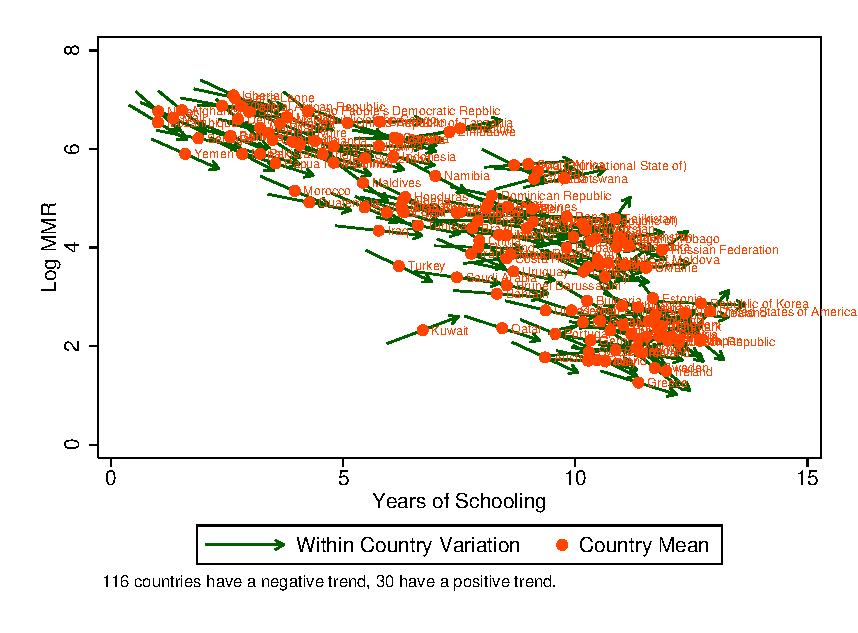
\includegraphics[scale=0.62]{./figures/countries}  
\caption{Between and Within Country Correlations: Education and MMR}
\end{figure}
\end{frame}

\begin{frame}[label=MMRnote]
\begin{center}
\begin{equation}
MMR=\frac{\text{deaths relating to pregnancy}}{100,000 \text{ live births}}
\end{equation}
\vspace{5mm}
\begin{equation}
MMRate=\frac{\text{deaths relating to pregnancy}}{\text{Women of Fertile Age}}
\end{equation}
\end{center}
\vspace{8mm}
So\ldots
\begin{equation}
MMR = \frac{MMRate}{\text{Fertility per woman}}=\frac{\text{maternal deaths/woman}}{\text{live births/woman}}
\end{equation}
\hyperlink{DATA}{\beamergotobutton{Back}}
\end{frame}

\begin{frame}[label=SumStats]
\begin{table}[htpb!]\begin{center}
\caption{Summary Statistics - Cross Country}\label{MMRtab:sumstats}
\begin{tabular}{lccccc}
&&&&& \\ \toprule Variable&Obs&Mean&Std. Dev.&Min&Max\\\midrule 
Maternal Mortality&710.0&220.6&300.9&2.0&1900.0\\
ln(Maternal Mortality)&710.0&4.302&1.649&0.6931&7.55\\
GDP per capita&702.0&9190.0&13870.0&64.36&104500.0\\
ln(GDP per capita)&702.0&7.966&1.649&4.164&11.56\\
Immunization&690.0&84.75&15.9&18.0&99.0\\
Fertility&718.0&3.163&1.676&0.887&8.659\\
Percent Attended Births&450.0&77.29&27.59&-2.6e-06&100.0\\
Population (Millions) &670.0&40.49&144.0&0.09515&1338.0\\
Teen Births&670.0&55.68&46.12&2.796&220.6\\
Husband wants more kids than wife&290.0&0.2107&0.07437&0.05331&0.3843\\
Husband wants less kids than wife&290.0&0.07031&0.03495&0.01606&0.1858\\
\midrule\multicolumn{6}{l}{\textsc{Education - Female}} \\ 
 Total Years of Education&730.0&8.07&3.319&0.4692&13.99\\
Years of Primary Education&730.0&4.714&1.693&0.3421&8.907\\
Years of Secondary Education&730.0&2.963&1.754&0.04875&7.459\\
Years of Tertiary Education&730.0&0.3932&0.3744&7.15e-08&2.048\\
Percent Primary&730.0&23.83&17.44&0.02&77.85\\
Percent Secondary&730.0&45.97&23.88&1.203&95.65\\
Percent Tertiary&730.0&12.58&12.05&0.0&62.86\\
Percent No Education&730.0&17.61&23.4&0.0&93.59\\
Male/Female Education (years)&730.0&1.16&0.4165&0.7114&4.499\\
\midrule
\multicolumn{6}{p{13.4cm}}{\begin{footnotesize}\textsc{Notes:} Maternal mortality is expressed in terms of    deaths per 100,000 live births. Immunization is expressed as the percent of   children of ages 12-23 months who are immunized against diphtheria, pertussis  and tetanus (DPT). Fertility represents births per woman, and teen births are expressed as the number of births per 1000 women between the ages of 15--19. Husband and wife fertility preferences are only available for DHS countries.\end{footnotesize}} \\ \bottomrule \end{tabular}\end{center}\end{table}
\hyperlink{DATA}{\beamergotobutton{Back}}
\end{frame}

\begin{frame}[label=SumStatsCountry]
\begin{table}[htpb!]											
\begin{center}											
\caption{Summary Statistics -- Natural Experiments}											
\label{MMRtab:sumstatsexperiment}											
\begin{tabular}{l c c c c c}											
& & & & & \\											
\toprule											
Variable	&	Obs	&	Mean	&	Std. Dev.	&	Min	&	Max	\\
\midrule
\multicolumn{6}{l}{\textsc{Panel A – Nigeria}}  \\											
Years of Education	&	13221	&	4.822	&	5.349	&	0	&	22	\\
Investment per Capita	&	12748	&	0.881	&	0.545	&	0.014	&	2.195	\\
Non-West State	&	13235	&	0.828	&	0.377	&	0	&	1	\\
Year of Birth (education)	&	13235	&	1968.329	&	5.119	&	1956	&	1975	\\
Maternal Mortality	&	25354	&	0.019	&	0.137	&	0	&	1	\\
Under 25 Maternal Mortality	&	29676	&	0.006	&	0.074	&	0	&	1	\\
Year of Birth (MM)	&	29967	&	1968.472	&	5.381	&	1956	&	1975	\\
\midrule											
\multicolumn{6}{l}{\textsc{Panel B – Zimbabwe}}  \\											
Years of Education	&	10195	&	7.023	&	3.788	&	0	&	21	\\
High School Enrollment	&	10195	&	0.439	&	0.496	&	0	&	1	\\
Treated	&	10201	&	0.622	&	0.485	&	0	&	1	\\
Year of Birth (education)	&	10201	&	1966.128	&	4.786	&	1956	&	1974	\\
Maternal Mortality	&	23699	&	0.013	&	0.115	&	0	&	1	\\
Under 25 Maternal Mortality	&	28631	&	0.003	&	0.055	&	0	&	1	\\
Year of Birth (MM)	&	28842	&	1966.023	&	4.736	&	1957	&	1974	\\
\midrule											
\multicolumn{6}{l}{\textsc{Panel C – Kenya}}  \\											
Years of Education	&	13712	&	7.168	&	4.149	&	0	&	23	\\
Treated	&	13712	&	0.575	&	0.443	&	0	&	1	\\
Year of Birth (education)	&	13712	&	1968.389	&	8.147	&	1950	&	1980	\\
Maternal Mortality	&	22738	&	0.014	&	0.116	&	0	&	1	\\
Under 25 Maternal Mortality	&	25616	&	0.006	&	0.076	&	0	&	1	\\
Year of Birth (MM)	&	25686	&	1967.686	&	7.770	&	1950	&	1980	\\
\midrule											
\multicolumn{6}{p{12cm}}{\begin{footnotesize}\textsc{Notes:}  Year of birth (education) refers to the birth cohorts of respondents to the DHS surveys for whom we observe educational attainment.  Year of birth (MM) refers to the birth cohorts in the maternal mortality data, who are sisters of DHS respondents.  In panel A investment per capita refers to federal funds dispersed for school construction in 1976 (in naira).  We do not observe this for the state Abuja which has existed since 1991 only.  In all panels maternal mortality and under 25 maternal mortality refers deaths due to pregnancy divided by the total number of women. \end{footnotesize}} \\											
\bottomrule											
\end{tabular}											
\end{center}											
\end{table}											


\hyperlink{DATA}{\beamergotobutton{Back}}
\end{frame}



\begin{frame}[label=otherPANEL]
  \begin{table}[htpb!]

    \begin{center}
     \scalebox{0.52}{
      \begin{tabular}{lcccccccc}\toprule

        &(1)&(2)&(3)&(4)&(5)&(6)&(7)&(8)\\

        VARIABLES&MMR&MMR&MMR&MMR&MMR&MMR&MMR&MMR\\\midrule

        \vspace{4pt}&\begin{footnotesize}\end{footnotesize}&\begin{footnotesize}\end{footnotesize}&\begin{footnotesize}\end{footnotesize}&\begin{footnotesize}\end{footnotesize}&\begin{footnotesize}\end{footnotesize}&\begin{footnotesize}\end{footnotesize}&\begin{footnotesize}\end{footnotesize}&\begin{footnotesize}\end{footnotesize}\\

        Years of Education&-233.0***&-236.5***&-207.1***&-206.3***&-191.5***&-185.4***&-191.9***&-184.4***\\

        & \begin{footnotesize}(23.83)\end{footnotesize} & \begin{footnotesize}(26.67)\end{footnotesize} & \begin{footnotesize}(24.03)\end{footnotesize} & \begin{footnotesize}(23.55)\end{footnotesize} & \begin{footnotesize}(26.85)\end{footnotesize} & \begin{footnotesize}(29.12)\end{footnotesize} & \begin{footnotesize}(37.32)\end{footnotesize} & \begin{footnotesize}(36.65)\end{footnotesize} \\

        Years of Education Squared&12.34***&12.51***&12.53***&12.49***&11.68***&11.44***&11.73***&11.31***\\

        & \begin{footnotesize}(1.347)\end{footnotesize} & \begin{footnotesize}(1.567)\end{footnotesize} & \begin{footnotesize}(1.522)\end{footnotesize} & \begin{footnotesize}(1.490)\end{footnotesize} & \begin{footnotesize}(1.581)\end{footnotesize} & \begin{footnotesize}(1.672)\end{footnotesize} & \begin{footnotesize}(2.040)\end{footnotesize} & \begin{footnotesize}(2.026)\end{footnotesize} \\

        year==1995&&&-8.620&-9.644&-4.161&-4.580&-6.012&-8.210\\

        & \begin{footnotesize}\end{footnotesize} & \begin{footnotesize}\end{footnotesize} & \begin{footnotesize}(10.81)\end{footnotesize} & \begin{footnotesize}(12.35)\end{footnotesize} & \begin{footnotesize}(12.01)\end{footnotesize} & \begin{footnotesize}(11.68)\end{footnotesize} & \begin{footnotesize}(13.14)\end{footnotesize} & \begin{footnotesize}(13.64)\end{footnotesize} \\

        year==2000&&&-25.12*&-26.49&-17.91&-17.58&-20.62&-21.82\\

        & \begin{footnotesize}\end{footnotesize} & \begin{footnotesize}\end{footnotesize} & \begin{footnotesize}(14.71)\end{footnotesize} & \begin{footnotesize}(16.99)\end{footnotesize} & \begin{footnotesize}(15.91)\end{footnotesize} & \begin{footnotesize}(16.01)\end{footnotesize} & \begin{footnotesize}(18.89)\end{footnotesize} & \begin{footnotesize}(19.10)\end{footnotesize} \\

        year==2005&&&-50.16***&-54.36**&-37.12*&-38.49*&-42.52*&-40.69\\

        & \begin{footnotesize}\end{footnotesize} & \begin{footnotesize}\end{footnotesize} & \begin{footnotesize}(17.23)\end{footnotesize} & \begin{footnotesize}(24.80)\end{footnotesize} & \begin{footnotesize}(22.21)\end{footnotesize} & \begin{footnotesize}(21.47)\end{footnotesize} & \begin{footnotesize}(25.56)\end{footnotesize} & \begin{footnotesize}(25.21)\end{footnotesize} \\

        year==2010&&&-75.56***&-82.38**&-64.34**&-65.31**&-69.95**&-63.63*\\

        & \begin{footnotesize}\end{footnotesize} & \begin{footnotesize}\end{footnotesize} & \begin{footnotesize}(21.61)\end{footnotesize} & \begin{footnotesize}(34.77)\end{footnotesize} & \begin{footnotesize}(30.85)\end{footnotesize} & \begin{footnotesize}(30.36)\end{footnotesize} & \begin{footnotesize}(34.74)\end{footnotesize} & \begin{footnotesize}(34.07)\end{footnotesize} \\

        log GDP per capita&&&&6.023&3.976&6.519&7.607&6.602\\

        & \begin{footnotesize}\end{footnotesize} & \begin{footnotesize}\end{footnotesize} & \begin{footnotesize}\end{footnotesize} & \begin{footnotesize}(17.30)\end{footnotesize} & \begin{footnotesize}(16.38)\end{footnotesize} & \begin{footnotesize}(15.60)\end{footnotesize} & \begin{footnotesize}(15.89)\end{footnotesize} & \begin{footnotesize}(16.02)\end{footnotesize} \\

        Immunization (DPT)&&&&&-1.843*&-1.765**&-1.818**&-1.812**\\

        & \begin{footnotesize}\end{footnotesize} & \begin{footnotesize}\end{footnotesize} & \begin{footnotesize}\end{footnotesize} & \begin{footnotesize}\end{footnotesize} & \begin{footnotesize}(0.934)\end{footnotesize} & \begin{footnotesize}(0.885)\end{footnotesize} & \begin{footnotesize}(0.867)\end{footnotesize} & \begin{footnotesize}(0.873)\end{footnotesize} \\

        Attended Births&&&&&&-0.636&-0.740&-0.870\\

        & \begin{footnotesize}\end{footnotesize} & \begin{footnotesize}\end{footnotesize} & \begin{footnotesize}\end{footnotesize} & \begin{footnotesize}\end{footnotesize} & \begin{footnotesize}\end{footnotesize} & \begin{footnotesize}(0.841)\end{footnotesize} & \begin{footnotesize}(0.827)\end{footnotesize} & \begin{footnotesize}(0.833)\end{footnotesize} \\

        Fertility&&&&&&&-9.667&-15.13\\

        & \begin{footnotesize}\end{footnotesize} & \begin{footnotesize}\end{footnotesize} & \begin{footnotesize}\end{footnotesize} & \begin{footnotesize}\end{footnotesize} & \begin{footnotesize}\end{footnotesize} & \begin{footnotesize}\end{footnotesize} & \begin{footnotesize}(22.73)\end{footnotesize} & \begin{footnotesize}(23.58)\end{footnotesize} \\

        Teen births&&&&&&&&0.793\\

        & \begin{footnotesize}\end{footnotesize} & \begin{footnotesize}\end{footnotesize} & \begin{footnotesize}\end{footnotesize} & \begin{footnotesize}\end{footnotesize} & \begin{footnotesize}\end{footnotesize} & \begin{footnotesize}\end{footnotesize} & \begin{footnotesize}\end{footnotesize} & \begin{footnotesize}(0.895)\end{footnotesize} \\

        Constant&1,163***&1,183***&981.7***&933.1***&1,038***&1,030***&1,097***&1,057***\\

        & \begin{footnotesize}(95.07)\end{footnotesize} & \begin{footnotesize}(105.2)\end{footnotesize} & \begin{footnotesize}(99.20)\end{footnotesize} & \begin{footnotesize}(156.1)\end{footnotesize} & \begin{footnotesize}(147.2)\end{footnotesize} & \begin{footnotesize}(145.3)\end{footnotesize} & \begin{footnotesize}(212.5)\end{footnotesize} & \begin{footnotesize}(226.8)\end{footnotesize} \\

        \vspace{4pt} & \begin{footnotesize}\end{footnotesize} & \begin{footnotesize}\end{footnotesize} & \begin{footnotesize}\end{footnotesize} & \begin{footnotesize}\end{footnotesize} & \begin{footnotesize}\end{footnotesize} & \begin{footnotesize}\end{footnotesize} & \begin{footnotesize}\end{footnotesize} & \begin{footnotesize}\end{footnotesize} \\

        Observations&710&428&428&428&428&428&428&428\\

        $R^2$&0.425&0.538&0.580&0.580&0.601&0.604&0.604&0.606\\

        Number of Countries&142&108&108&108&108&108&108&108\\ \midrule

        \multicolumn{9}{c}{\begin{footnotesize} *** p$<$0.01, ** p$<$0.05, * p$<$0.1\end{footnotesize}} \\
        \multicolumn{9}{p{19cm}}{\begin{footnotesize}\textsc{Notes:} All regressions include fixed-effects by country.  Results are for average years of education of females between the ages of 15 and 39 in each country.  A full description of control variables is available in section 6. \end{footnotesize}} \\
        \bottomrule
      \end{tabular}
      }
    \end{center}
  \end{table}
\hyperlink{PTABLE}{\beamergotobutton{Back}}
\end{frame}


\begin{frame}[label=ZIMBABWE]
Follow Ag\"uero and Bharawadj (2011) in estimating around the discontinuity in educational
attainment between 14 and 15 year old cohorts in 1980:
\vspace{5mm}
\begin{eqnarray}
 \label{eqn:Zimbabwe}
 y_{ij}&=&\beta_1\text{DumAge}_{ij}+\beta_2\text{DumAge}_{ij}\times(\text{Age}80_{ij}-14)+ \\ \nonumber
 && \beta_3(1-\text{DumAge}_{ij})\times(\text{Age}80_{ij}-14)+\textbf{X}^\prime_{ij}\theta+\varepsilon_{ij}.
\end{eqnarray}
\vspace{5mm}
\hyperlink{ID}{\beamergotobutton{Back}}
\end{frame}

\begin{frame}[label=KENYA]
As per Chicoine (2011) define treatment based on probability of being in an affected
cohort, and fit flexible quarter-of-birth trends:
\vspace{5mm}
\begin{equation}
\label{eqn:Kenya}
 y_{ijq}=\alpha+\beta\text{Treat}_{jk}+\textbf{age}_{ijq}^\prime\gamma+\textbf{qob trend}_{jq}^\prime \delta +\textbf{X}^\prime_{ijq}\theta+\varepsilon_{ijq},
\end{equation}
\vspace{5mm}
\hyperlink{ID}{\beamergotobutton{Back}}
\end{frame}


\begin{frame}[label=NIGERIA_EDUC]
\begin{figure}[!htbp]
\begin{center}
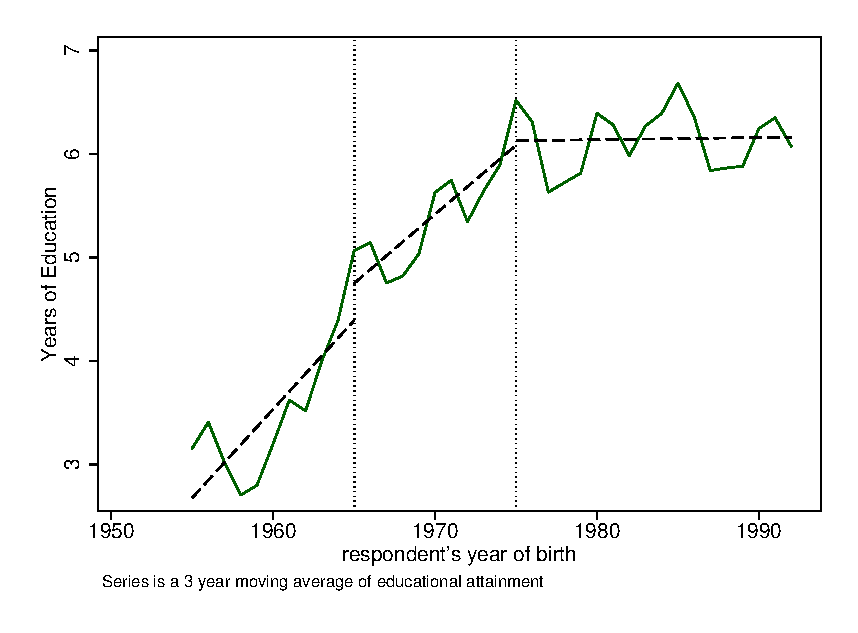
\includegraphics[scale=0.7]{./figures/Nigeria_educ.eps}
\caption{Educational Attainment by Cohort: Nigeria}
\end{center}
\end{figure}
\hyperlink{ZIMBABWE_EDUC}{\beamergotobutton{Back}}
\end{frame}

\begin{frame}[label=NIGERIA_MMR]
\begin{figure}[!htbp]
\begin{center}
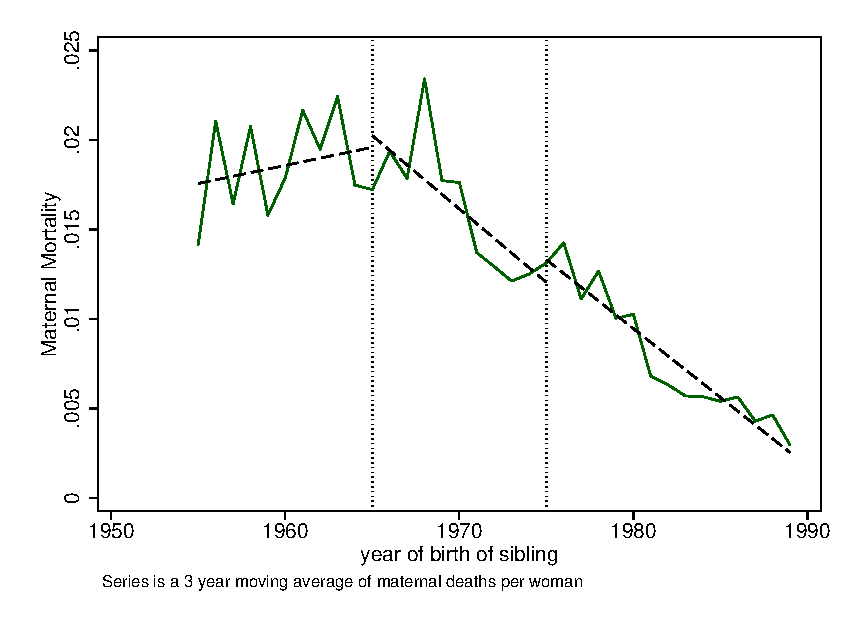
\includegraphics[scale=0.7]{./figures/Nigeria_mmr.eps}
\caption{Maternal Mortality by Cohort: Nigeria}
\end{center}
\end{figure}
\hyperlink{ZIMBABWE_MMR}{\beamergotobutton{Back}}
\end{frame}


\end{document}

In panel A, `Final birth twins' refers to those families where twins occur on their last birth and those families with an identical number of births but one 
fewer child due to singleton births.  All children (both in twin and non-twin families) are considered pre-twin if they are born before the final birth.  In panel B, `Twins
exceeding desired quantity' refers to those families where a twin birth on the final birth causes parents to exceed their optimal number of children, and similar families who
achieve optimal fertility levels with singleton final births.
